\documentclass[10pt]{article}
% Preamble to the document, to avoid cluttering it up

\title{Smarter Code Autocomplete}
\author{
    \textsc{James Gippetti}
        \qquad
    \textsc{Adrien Fallou}
        \qquad
    \textsc{Susan Tu}
        \mbox{}\\ %
        \\
        CS221\\
        \mbox{}\\ %
        \normalsize
            \texttt{jgippetti}
        \textbar{}
            \texttt{afallou}
        \textbar{}
            \texttt{sctu}
        \normalsize
            \texttt{@stanford.edu}
}
\date{\today}

%\documentclass{acmconf}
%\usepackage[pdftex]{graphicx}

\usepackage{amsmath}
\usepackage{listings}
\usepackage{xcolor}
%\usepackage[paper=a4paper,dvips,top=1.5cm,left=1cm,right=1cm,
%   foot=2.5cm,bottom=2.5cm]{geometry}


% listings magic!
\definecolor{DefaultColor}{HTML}{00428C}
\definecolor{CommentColor}{HTML}{60A0B0}
\definecolor{BackgroundColor}{HTML}{E4E5E7}
\definecolor{FrameColor}{HTML}{95ABD0}
\definecolor{NumberColor}{HTML}{40A070}
\definecolor{IDColor}{HTML}{06278E}
\definecolor{KeywordColor}{HTML}{007020}
\definecolor{TypeColor}{HTML}{902000}


% Courtesy of% http://tex.stackexchange.com/questions/34896/coloring-digits-with-the-listings-package
\newcommand\digitstyle{\color{NumberColor}}\makeatletter\newcommand{\ProcessDigit}[1]{%
  \ifnum\lst@mode=\lst@Pmode\relax%
   {\digitstyle #1}%
  \else
    #1%
  \fi
}
\makeatother
\lstset{literate=
    {0}{{{\ProcessDigit{0}}}}1
    {1}{{{\ProcessDigit{1}}}}1
    {2}{{{\ProcessDigit{2}}}}1
    {3}{{{\ProcessDigit{3}}}}1
    {4}{{{\ProcessDigit{4}}}}1
    {5}{{{\ProcessDigit{5}}}}1
    {6}{{{\ProcessDigit{6}}}}1
    {7}{{{\ProcessDigit{7}}}}1
    {8}{{{\ProcessDigit{8}}}}1
    {9}{{{\ProcessDigit{9}}}}1
}

\lstset{
    backgroundcolor=\color{BackgroundColor},
    basicstyle=\color{DefaultColor}\footnotesize\tt,
    breakatwhitespace=false,
    breaklines=true,
    commentstyle=\color{CommentColor}\textsl,
    frame=true,
    frameshape={yyy}{y}{y}{yyy},
    identifierstyle=\color{IDColor},
    keywordstyle=\color{KeywordColor},
    language=Haskell,
    emph={Bool, Char, String, IO, Maybe, Either, Ordering, Int, Integer, Ratio, Float, Double, Complex, TVar, MVar, STM},
    emphstyle=\color{TypeColor},
    rulecolor=\color{FrameColor},
    rulesepcolor=\color{FrameColor},
    showstringspaces=false,
    stringstyle=\color{FrameColor}, % apparently
    tabsize=2
}

% end of listings magic

\usepackage[margin=2.5cm]{geometry}
\usepackage{float}
\usepackage{multicol}
\usepackage[pdftex]{graphicx}
\usepackage[english]{babel}
\usepackage{sidecap}
\usepackage[font=small,labelfont=bf]{caption}
\usepackage[raggedright]{titlesec}
\usepackage{hyperref}

\makeatletter
\newenvironment{tablehere}
  {\def\@captype{table}}
  {}

\newenvironment{figurehere}
  {\def\@captype{figure}}
  {}
\makeatother

\begin{document}
\maketitle

		Most programmers use autocompletion tools to write code faster. However, basic language-agnostic autocomplete tools (for example, what comes pre-installed with VIM 7.3) suffer from two weaknesses: 1) they only complete one word at a time, and 2) they complete the current word by matching leading characters. Our project is motivated by the popularity of more advanced autocompletion plugins such as Jedi (for Python autocompletion)[1] and Visual Studio’s Intellisense. Our goal is to provide smart, language-agnostic autocomplete. We demonstrate this strategy by building a tool that provides autocomplete for the Python programming language. We then discuss how our model can apply to other languages.

\section{Approach}
 
		Our initial strategy was to try and predict the next keyword that the programmer would type before she started entering the character sequence of that keyword using an n-grams approach. Exploring this approach showed us its limitations: 1) we are still predicting one word at a time and 2) because it is a very global, the predictions that this model output were of little practical value for the programmer.
        
        Attempting to address 1) led us to explore a factor graph approach (where each assignment might be equivalent to a prediction), and find that approach had been explored by Han et. al. at MIT \cite{han}. Another approach that completes multiple words at a time is presented in "Keyword Programming" \cite{little}, where the words do not even have to be in order; However, the approach described in this paper seemed more difficult to generalize to other programming languages, since their approach had knowledge of Java-specific notions of \texttt{static}, generics, etc.

	Consequently, our refocused efforts have been based on Han et. al.'s approach: We aim to autocomplete a whole sequence of keywords at once based on a partial input, and one of our additions to the model presented in Han et. al. addresses 2).

\section{Modified HMM Model}

\begin{figure}[h]
  \centering
    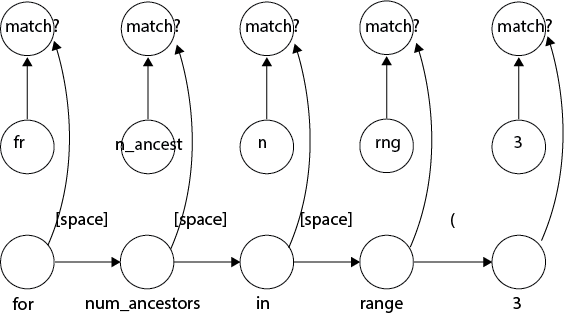
\includegraphics[scale=0.3]{HMM.png}
  \caption{HMM Model with emission probabilities replaced by match probabilities.}
\label{fig:sparselog}
\end{figure}

The Han paper \cite{han} uses a Hidden Markov Model (HMM). In this model, the user must correctly input separators between abbreviated names. Here `names' refers to names of functions, classes, variables, as well as keywords in the language. We also use 'names' to refer to string literals and numerical constants, but we treat these specially; we do not attempt to un-abbreviate these. Our notion of names is dependent on our choice of language (Python) but in our discussion of our implementation, we will discuss how our approach can be generalized to other programming languages given a lexer and a parser for that language. 

	As an example (illustrated in Figure 1), the user may input \texttt{fr n\_ancest n rng(3):}. We treat each of the abbreviated names, \texttt{fr}, \texttt{n\_ancest}, \texttt{n}, \texttt{rng}, and \texttt{3}, as the emissions in a Hidden Markov Model. We consider the full names corresponding to the abbreviated input as the assignment to the hidden states that we are trying to find. Although we use the term "abbreviated," the names the user enters are not restricted to abbreviations of the correct names. We expect to be able to correct for misspellings involving extra characters as well.

\subsection{Match Probabilities}

The standard HMM model is not perfectly suited to our use case. In a standard HMM model, we need to estimate $P(\texttt{fr} | \texttt{for})$ and we need to guarantee that $\sum_{s \in S} P(\texttt{fr}|s)=1$ where $S$ is the set of all names observed in the existing codebase. However, there are infinitely many permutations of characters that could be attempts to abbreviate \texttt{for}, so it is unclear how we would estimate the probabilities that we would need to solve the HMM. Han, et. al. propose replacing the emission probability with a match probability. The domain for this match node (i.e., the top-most row of nodes in Figure 1) is $\{0,1\}$, and the probability associated with the transitions to them is $P(y=1 | t=\texttt{fr}, s=\texttt{for})$, where $y$ is the value of the match node, $t$ is the value of the emission, and $s$ is the value of the hidden state.

Han et. al.,  obtain the probabilities for the match nodes by treating the assignment of the hidden state as a multiclass classification problem. There they let $ p(y | t, s)=P_L(t|s)$ where $P_L$ is the probabiity according the prediction of a multiclass logistic regression classifier. They choose logistic regression because the probabilities at any one node, after summing over all possible hidden states, sums to 1, which is what we wanted for the emission probabilties in the standard HMM Model. 

\subsection{State-to-state Transition Probabilities}

The transition probability from state $s_i$ to $s_{i+1}$ is
\[
	p(s_{i+1} | s_i) = \lambda*T(s_i,c_{i+1},s_{i+1}) + \lambda*T(s_i)
\]
Where $T(s_i,c_{i+1},s_{i+1})$ is the proportion of times that $s_i$ followed by $c_{i+1}$ is followed by $s_{i+1}$ and $T(s_i)$ is the proportion of times that statements start with $s_i$. Note that we do not simply use $T(s_i,c_{i+1},s_{i+1})$ for the transition probabilities because it is possible that $s_i$ followed by $c_{i+1}$ has never been seen before. $\lambda$ is some constant that should be tuned; Han et. al. use 0.7. 

Therefore the expression that we are trying to maximize for this modified HMM Model is essentially the same as for the standard HMM model, the only difference being the replacement of the emission probabilities with match probabilities. Where $T$ is the total number of hidden states and $c_i$ is the separator that appears before the $i$th abbreviated name, $P(t_1,\ldots, t_T, s_1,\ldots,s_T, c_2,\ldots,c_T)=T(s_1)\prod_{t=1}^{T-1} T(s_i,c_{i+1}, c_{s+1})\prod_{t=1}^{T}P(y=1|s_i,t_i)$. (However, recall that we do not try to correct string literals or numerical constants; therefore we use some constant value for the transition to such a state and 1.0 for the match probability.)

\section{Algorithm}

	We use the Viterbi algorithm to find the most likely state sequence.
We denote our state space as $S$. If we have initial probability $\pi_i$ of being in state $i$ and transition probability $t_{i,j}$ of going from state $i$ to $j$, then the most likely sequence $h_1, h_2, ..., h_T$ for the hidden variable given observations $e_1, e_2, ..., e_T$ is given by the recurrence relation:
    \[
    	\begin{cases}
        	V_{1,k} = P(e_1|k).\pi_k \\
            V_{t,k} = P(e_t | k) \underset{h \in S}\max(t_{h,k}.V_{t-1,h})
        \end{cases}
    \]
    Where $V_{t,k}$ is the probability of the most probable state sequence responsible for the first $t$ observations, that has $k$ as its final state. We then find the solution to this recurrence using dynamic programming, and find the most likely path by keeping track of the argmax.

	In our case, we want to have $n$ suggestions, we can either modify Viterbi to keep track of the $n$ best assignments, or, if Viterbi turns out to be quite slow becuase we have too many possible names that each state could be, we can obtain the $n$ highest probability assignments using particle filtering.
    
\section{Improvements}

Our contributions to the model in Han et. al.'s paper is two-fold. We plan to improve the match probability estimations by incorporating locality into the features used with the logistic regression classifier. In addition, the original modified HMM Model considers only the probability of transitioning into a state given the previous state; it does not consider even earlier states, which may lead to the suggestion of states sequences that do not parse correctly. For example, \texttt{with open(dirpath,rw\_mode) and} does not parse correctly but could be suggested if \texttt{rw\_mode}) is followed by \texttt{and} in some previous snippet of code. Our improvement will ensure that we never suggest a statement that does not parse correctly.  

\subsection{Prefixes of Valid Parses}

\begin{figure}[h]
  \centering
    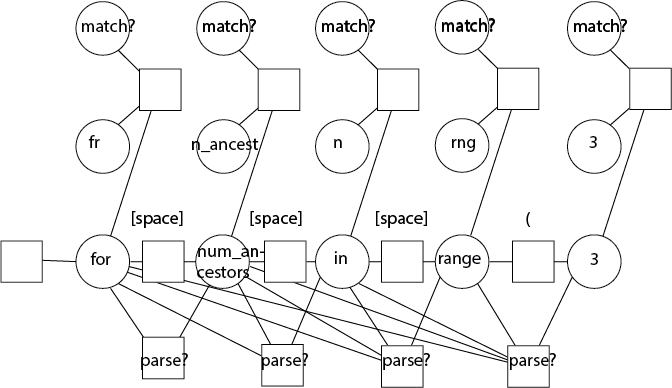
\includegraphics[scale=0.3]{improvedFactorGraph.png}
  \caption{Factor graph representation of our model.}
\label{fig:sparselog}
\end{figure}

The nodes in Figure 2, which is otherwise a factor graph representation of Figure 1, labeled 'parse?' have domains $\{0,1\}$, and their value is 1 if and only if the statement up to that point is a prefix of a valid parse. In the context of the example presented in the figure, the 'parse?' nodes, from left to right, ensure that for any assignment with nonzero weight, we have that $s_1 c_2 s_2$ is a prefix of a valid parse,   $s_1 c_2 s_2 c_3 s_3$ is a prefix of a valid parse, $s_1 c_2 s_2  c_3 s_3 c_4 s_4$ is a prefix of a valid parse, etc. 

\subsection{Locality}

The features that are used in the paper do not take locality into consideration and purely assess the match based on the letters present in the value that we are considering assigning to the state and the letters present in the emission. However, it seems to make intuitive sense that if in the present file we have often typed \texttt{arg2} after \texttt{arg1,}, we should suggest arg2 after \texttt{arg1,}, even if in another, unrelated context (where \texttt{arg1} may not be a data structure of the same type that it is in the current context)\texttt{arg1,} was often followed by \texttt{arg3}. We plan on trying the features in Table 1 and adding/removing features as needed.
\\\\
\begin{tablehere}
\begin{tabular}{c c c} 
\hline
Inputs & feature & \\
\hline % inserts single horizontal line
$s$,$t$ & number of consonant letter matches\\ % inserting body of the table
$s$,$t$ & number of capitalized latter matches\\
$s$,$t$ & number of non-alphabet character matches\\
$s$,$t$ & number of letter matches, ordering ignored \\
$s$,$t$ & number of letter matches, ordering enforced \\
$s$,$t$ & percentage of matched capital letters in $s$ \\ 
$s$,$t$ & percentage of matched consonant letters in $s$ \\
$s$,$t$ & percentage of matched letters in $s$ \\
$s$,$t$ & percentage of matched letters in $x$ \\
$s$,$t$,$filename_s$, $filename_t$ & whether $filename_s=filename_t$ \\
$s$, $t$, $lineno_s$, $lineno_t$ & $|lineno_s-lineno_t|$ if $filename_s=filename_t$ else the number of lines in the longest file\\
\end{tabular}
\caption{Features for logistic regression. The first nine, which depend solely on $s$ and $t$, are taken from Han et. al.'s paper. The last two are our addition.\\\\}
\end{tablehere}


In order to get a training examples, we will pick a random line in the source code and generate an abbreviated version of the line (some simple, automatable, strategies we could use might be to remove all vowels, randomly insert a few letters to simulate typing errors from the user, etc.) For each name in the line, we now have a name $s$ and an abbreviated name $t$. Consider all other occurences of $s$ in the codebase (except for those that come after the randomly chosen line in the same file as that line); suppose there are $k$ such occurrences $o_1, o_2,\ldots, o_k$ (each of which is associated with a line number and filename). We can now train on $k$ inputs ($t,o_1$), ($t,o_2$),...,($t,o_k$), where the label for all of them is $s$. As an example, consider the penultimate feature in the table and our example name \texttt{num\_ancestors}. Intuitively, in training, if we see that \texttt{n\_ancest} appears only in the same file as \texttt{num\_ancestors}, then in classification, if this feature evaluates to 1, this feature will increase the probability of \texttt{n\_ancest} being classified as \texttt{n\_ancestor}.

\section{Implementation Details}
 
We have implementated the creation of the transition probabilites in the HMM, but have yet to complete the logistic regression for the match probabilities. For the separators used for the transition probabilities, we are consolidating consecutive separators, so if there are multiple separators in a row--for example \texttt{,**} in \texttt{some\_method(self,**kwargs)}--our model will just treat \texttt{,**} as one separator.

Note that from the way we have described the model, algorithm, and implementation, we can see that our overall strategy could be generalized to any language for which we have a lexer and a parser. (In Python, these are provided in the \texttt{tokenizer} and \texttt{parser} modules.) We need only to specify which types of tokens returned by the lexer should be considered separators, which should be considered names, and which (i.e., comments) should be ignored; in all other respects the implementation remains the same. 

\section{Comparison with Baseline \& Oracle}
For our initial proposal we wrote a simple n-gram model to predict the next keyword based on previous keywords. (We achieved only $0.8\%$ accuracy with bigrams.) Since we have revised our strategy since the proposal, we also revised our baseline to be the model proposed and implemented in the Han paper. Based on their results, Han et. al. were able achieve an average accuracy of 80.2\% when comparing the top 1 recommended sequence of keywords to the original sequence and as high 94.5\% for the top 3 and 97.3\% for the top 5 (\cite{han}). We are curious as to whether we can achieve similarily encouraging results on Python codebases. (Han et. al. ran their model exclusively on Java codebases.) By implementing our proposed improvements to their model, we hope to surpass the performance of their model on Python codebases. For our oracle, we are still using the programmer, who obviously knows his own intended sequence of names. Even though this task is straightforward for our oracle, it affirms the feasibility of the task at hand.
\begin{thebibliography}{9}

\bibitem{jedi} \url{https://github.com/davidhalter/jedi-vim}

\bibitem{han} Han, S., Wallace, D.R., and Miller, R.C. Code Completion From Abbreviated Input. \emph{IEEE/ACM International COnference on Automated Software Engineering}, 332-43, 2009.

\bibitem{little} G. Little and R.C. Miller, "Keyword programming in Java," In Proc. ASE, vol. 16, pp. 37-71, 2007.

\end{thebibliography}


\end{document}
\end{document}